\documentclass[tikz,border=2pt]{standalone}
\usepackage{amsmath,amssymb}
\usepackage{tikz}
\usetikzlibrary{arrows.meta}

\begin{document}
% The solution set of two linear equations in the plane: one point, no point, or a whole line.
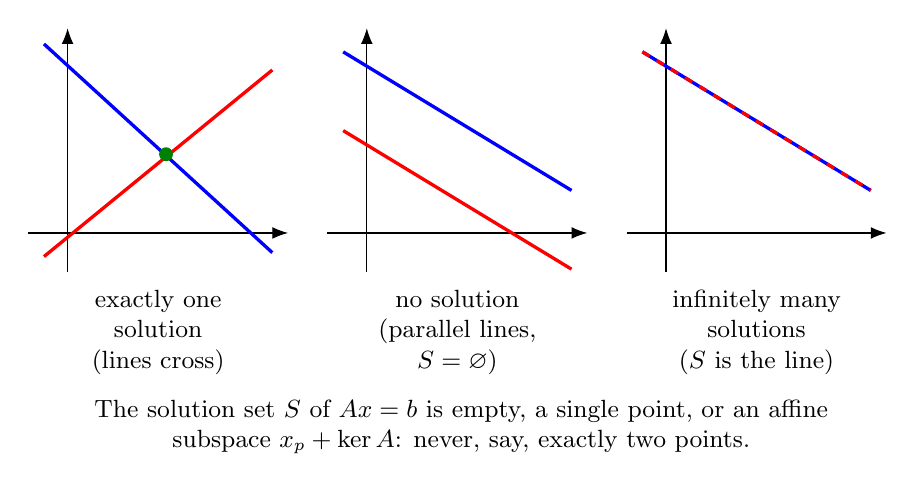
\begin{tikzpicture}[every node/.style={font=\small}, >={Latex[length=2mm]}]
	\begin{scope}
		\draw[->] (-0.5,0) -- (2.8,0);
		\draw[->] (0,-0.5) -- (0,2.6);
		\draw[blue, very thick] (-0.3,2.4) -- (2.6,-0.25);
		\draw[red, very thick] (-0.3,-0.3) -- (2.6,2.07);
		\fill[green!50!black] (1.25,1.0) circle (2.5pt);
		\node[anchor=north, align=center] at (1.15,-0.6) {exactly one\\ solution\\ (lines cross)};
	\end{scope}
	\begin{scope}[xshift=3.8cm]
		\draw[->] (-0.5,0) -- (2.8,0);
		\draw[->] (0,-0.5) -- (0,2.6);
		\draw[blue, very thick] (-0.3,2.3) -- (2.6,0.54);
		\draw[red, very thick] (-0.3,1.3) -- (2.6,-0.46);
		\node[anchor=north, align=center] at (1.15,-0.6) {no solution\\ (parallel lines,\\ $S=\varnothing$)};
	\end{scope}
	\begin{scope}[xshift=7.6cm]
		\draw[->] (-0.5,0) -- (2.8,0);
		\draw[->] (0,-0.5) -- (0,2.6);
		\draw[blue, very thick] (-0.3,2.3) -- (2.6,0.54);
		\draw[red, very thick, dashed] (-0.3,2.3) -- (2.6,0.54);
		\node[anchor=north, align=center] at (1.15,-0.6) {infinitely many\\ solutions\\ ($S$ is the line)};
	\end{scope}
	\node[anchor=north, align=flush center, text width=10cm] at (5.0,-2.0) {The solution set $S$ of $Ax=b$ is empty, a single point, or an affine subspace $x_p+\ker A$: never, say, exactly two points.};
\end{tikzpicture}
\end{document}
